\RequirePackage{fix-cm}
\documentclass[titlepage]{article}

\usepackage[utf8]{inputenc}
\usepackage{fullpage}    % Use the whole page
\usepackage{fancyhdr}    % Nice headers/footers
%\usepackage{mdwlist}     % For itemize* and enumerate*
\usepackage{graphicx}    % Importing graphics
\usepackage{hyperref}    % Hyperlink references and URLs
\usepackage[figure,table]{hypcap} % Hyperlink points to the top of figures
\usepackage[usenames,dvipsnames]{xcolor}	% Logo
\usepackage{tikz,ifthen}			% Logo
\usepackage{pgf}				% Logo
\usepackage{scalefnt}				% Logo
\usepgfmodule{shapes}				% Logo
\usepgfmodule{plot}				% Logo
\usetikzlibrary{shapes,arrows,shadows,fit}
\usepackage{pgf-umlsd}
\usepackage{multirow}
\usepackage{mdwlist}
\usepackage{colortbl}
\usepackage{calc}

\renewenvironment{itemize*}%
    {\begin{itemize}%
        \setlength{\itemsep}{0pt}%
        \setlength{\parskip}{0pt}%
        \setlength{\partopsep}{0pt}%
        \setlength{\topsep}{0pt}}%
    {\end{itemize}}

\newcommand{\operations}[1]{
\begin{center}
    \begin{tabular}{|p{3cm}|p{9cm + 2.0\tabcolsep}|}
    \hline
    \multicolumn{2}{|l|}{\cellcolor[gray]{0.5}{\textbf{Operations}}} \\ \hline
#1
    \end{tabular}
\end{center}
}
\newcommand{\operation}[4]{
    \hline
    \multicolumn{2}{|l|}{\cellcolor[gray]{0.8}{\texttt{#1}}} \\ \hline
    \hspace{7pt}\textbf{Input:} & #2 \\ \hline
    \hspace{7pt}\textbf{Output:} & #3 \\ \hline
    \hspace{7pt}\textbf{Description:} & #4 \\ \hline
}

\newcommand{\attributes}[1]{
    \begin{center}
        \begin{tabular}{|p{3cm}|p{2cm}|p{7cm}|}
            \multicolumn{3}{|l|}{\cellcolor[gray]{0.5}{\textbf{Attributes}}} \\ \hline
            \rowcolor[gray]{0.8} Name & Type & Description \\ \hline 
            #1
        \end{tabular}
    \end{center}
}

\newcommand{\attribute}[3]{
    \texttt{#1} & \texttt{#2} & #3 \\ \hline
}

% Just so we don't have to specify this twice
\newcommand\mytitle{Software Design Specification}
\newcommand\mydate{\today}
\newcommand\myversion{1}

\hypersetup{
    colorlinks=true,
    linkcolor=blue,
    urlcolor=blue,
    pdftitle={AHOY Software Design Specification V\myversion},
    pdfauthor={Dustin Ingram, Aaron Rosenfeld, Maria Kolakowska, Frank Clark}
}

% So we can number subsubsections too
\setcounter{secnumdepth}{5}

% For headers and footers
\setlength{\headheight}{15pt}
\setlength{\headsep}{25pt}
\pagestyle{fancy}
	
% Page style for the title page
\fancypagestyle{plain}{
    \fancyhf{}
    \renewcommand{\headrulewidth}{0pt}
    \renewcommand{\footrulewidth}{0pt}
}

% Page style for every other page
\fancyhf{} % clear all header and footer fields
\fancyhead[L]{AHOY}
\fancyhead[C]{\mytitle}
\fancyhead[R]{\mydate}
\fancyfoot[C]{\thepage}
\renewcommand{\headrulewidth}{0.4pt}
\renewcommand{\footrulewidth}{0.4pt}

\title{\textbf{\mytitle}}
\author{
	Frank Clark \\\url{francis.j.clark@drexel.edu}
    \and Dustin Ingram \\\url{dustin.s.ingram@drexel.edu}
	\and Maria Kolakowska \\\url{maria.j.kolakowska@drexel.edu}
    \and Aaron Rosenfeld \\\url{aaron.rosenfeld@drexel.edu}
}
\date{\mydate\\Version \myversion}

%%% Tikz stuff %%%
% Style for UML Class with attributes and methods
%BEGIN IMAGE
\tikzstyle{umlclass} = [
    rectangle, rectangle split, rectangle split parts=3,
    % This makes a nice gradient
    top color=white, bottom color=blue!30, draw=blue!50!black!100,
    drop shadow, rounded corners,
    node distance = 5cm, text width = 10cm, minimum width=10cm]
\tikzstyle{component} = [umlclass, rectangle split parts=0, text width =, node distance=3.14159cm, minimum width=]
% Line styles
\tikzstyle{hasa} = [draw, <-, >=open diamond]
\tikzstyle{ownsa} = [draw, ->, >=diamond]
\tikzstyle{isa} = [draw, ->, >=open triangle 45]

\newcommand{\umlclass}[5][,]{
    \node [umlclass,#1] (#2) {
        \textbf{#3}
        \nodepart{second}
        \begin{description*}
        #4
        \end{description*}
        \nodepart{third}
        \begin{description*}
        #5
        \end{description*}
    };
}

\newcommand{\eumlclass}[4][,]{
    \node [umlclass,#1] (#2) {
        \textbf{#3}
        \nodepart{second}
        \nodepart{third}
        \begin{description*}
        #4
        \end{description*}
    };
}

\newcommand{\umlattr}[3]{
    \item[$#1$]\textbf{#2}: \textit{#3}
}
\newcommand{\umlmethod}[4]{
    \item[$#1$]\textbf{#2}({#3}): \textit{#4}
}
\newcommand{\umlarg}[2]{\textit{#1} #2}

\newcommand{\umlrelation}[6][-|]{
    \path [#3] (#2) #1 (#4)
        node [very near start, auto=right] {#5}
        node [very near end, auto=right] {#6};
}
%END IMAGE
%%% End tikz stuff %%%

\begin{document}
\pagenumbering{roman}

\begin{figure*}
   % \vspace{-2em}
    \centering
    \scalebox{0.8}{
\begin{tikzpicture}[scale=1]
	
	\pgfsetlinewidth{3pt}

	% Background
	\color{cyan!70!black}
	\pgfpathmoveto{\pgfpointxy{-5}{2}}
	\pgfpathlineto{\pgfpointxy{-5}{11}}
	\pgfpathlineto{\pgfpointxy{-2}{11.9}}	
	\pgfpathlineto{\pgfpointxy{2}{11.9}}	
	\pgfpathlineto{\pgfpointxy{5}{11}}
	\pgfpathlineto{\pgfpointxy{5}{2}}
	\pgfpathclose 
	\pgfusepath{fill,stroke} 

	% Base
	\color{green!70!black}
	\pgfsetstrokecolor{black}
	\pgfpathmoveto{\pgfpointxy{-2}{1.5}}
	\pgfpathcurveto{\pgfpointxy{-2}{1.5}}{\pgfpointxy{-6}{1.5}}{\pgfpointxy{-6}{2.5}}
	\pgfpathlineto{\pgfpointxy{-6}{4}}
	\pgfpathlineto{\pgfpointxy{6}{4}}
	\pgfpathlineto{\pgfpointxy{6}{2.5}}
	\pgfpathcurveto{\pgfpointxy{6}{1.5}}{\pgfpointxy{2}{1.5}}{\pgfpointxy{2}{1.5}}
	\pgfpathclose 
	\pgfusepath{fill,stroke} 

	% Curtains
	\color{red!70!black}
	\pgfsetstrokecolor{black}

	% Left
	\pgfpathmoveto{\pgfpointxy{-6}{11}}
	\pgfpathlineto{\pgfpointxy{-6}{2.5}}
	\pgfpathcurveto{\pgfpointxy{-6}{2.2}}{\pgfpointxy{-3.5}{2.2}}{\pgfpointxy{-3.5}{2.5}}
	\pgfpathcurveto{\pgfpointxy{-3.5}{3}}{\pgfpointxy{-3.5}{4}}{\pgfpointxy{-4.5}{5}}
	\pgfpathcurveto{\pgfpointxy{-2.5}{7}}{\pgfpointxy{-4}{11}}{\pgfpointxy{-3}{11.5}}
	\pgfpathcurveto{\pgfpointxy{-4}{11}}{\pgfpointxy{-2.5}{7}}{\pgfpointxy{-4.5}{5}}
	\pgfpathcurveto{\pgfpointxy{-2.5}{7}}{\pgfpointxy{-6}{11}}{\pgfpointxy{-3}{11.5}}
	\pgfpathcurveto{\pgfpointxy{-6}{11}}{\pgfpointxy{-2.5}{7}}{\pgfpointxy{-4.5}{5}}
	\pgfpathcurveto{\pgfpointxy{-2.5}{7}}{\pgfpointxy{-8}{11}}{\pgfpointxy{-3}{11.5}}
	\pgfpathcurveto{\pgfpointxy{-8}{11}}{\pgfpointxy{-2.5}{7}}{\pgfpointxy{-4.5}{5}}
	\pgfpathcurveto{\pgfpointxy{-2.5}{7}}{\pgfpointxy{-2.5}{11}}{\pgfpointxy{-3}{11.5}}
	\pgfusepath{fill,stroke}

	% Right
	\pgfsetlinewidth{3pt}
	\pgfpathmoveto{\pgfpointxy{6}{11}}
	\pgfpathlineto{\pgfpointxy{6}{2.5}}
	\pgfpathcurveto{\pgfpointxy{6}{2.2}}{\pgfpointxy{3.5}{2.2}}{\pgfpointxy{3.5}{2.5}}
	\pgfpathcurveto{\pgfpointxy{3.5}{3}}{\pgfpointxy{3.5}{4}}{\pgfpointxy{4.5}{5}}
	\pgfpathcurveto{\pgfpointxy{2.5}{7}}{\pgfpointxy{4}{11}}{\pgfpointxy{3}{11.5}}
	\pgfpathcurveto{\pgfpointxy{4}{11}}{\pgfpointxy{2.5}{7}}{\pgfpointxy{4.5}{5}}
	\pgfpathcurveto{\pgfpointxy{2.5}{7}}{\pgfpointxy{6}{11}}{\pgfpointxy{3}{11.5}}
	\pgfpathcurveto{\pgfpointxy{6}{11}}{\pgfpointxy{2.5}{7}}{\pgfpointxy{4.5}{5}}
	\pgfpathcurveto{\pgfpointxy{2.5}{7}}{\pgfpointxy{8}{11}}{\pgfpointxy{3}{11.5}}
	\pgfpathcurveto{\pgfpointxy{8}{11}}{\pgfpointxy{2.5}{7}}{\pgfpointxy{4.5}{5}}
	\pgfpathcurveto{\pgfpointxy{2.5}{7}}{\pgfpointxy{2.5}{11}}{\pgfpointxy{3}{11.5}}
	\pgfusepath{fill,stroke}

	% Top
	%     Top-left
	\pgfpathmoveto{\pgfpointxy{-2}{12}}
	\pgfpathcurveto{\pgfpointxy{-2}{12}}{\pgfpointxy{-6}{12}}{\pgfpointxy{-6}{11}}
	\pgfpathcurveto{\pgfpointxy{-5}{9}}{\pgfpointxy{-2}{11}}{\pgfpointxy{-2}{11.85}}
	\pgfpathcurveto{\pgfpointxy{-2}{11.5}}{\pgfpointxy{-4.5}{9.5}}{\pgfpointxy{-6}{11}}
	\pgfpathcurveto{\pgfpointxy{-4.5}{9.5}}{\pgfpointxy{-2}{11.5}}{\pgfpointxy{-2}{11.85}}
	\pgfpathcurveto{\pgfpointxy{-2}{12}}{\pgfpointxy{-3.5}{10.4}}{\pgfpointxy{-6}{11}}
	\pgfpathcurveto{\pgfpointxy{-3.5}{10.4}}{\pgfpointxy{-2}{12}}{\pgfpointxy{-2}{11.85}}

	%    Top-middle
	\pgfpathcurveto{\pgfpointxy{-1}{10.5}}{\pgfpointxy{1}{10.5}}{\pgfpointxy{2}{11.85}}
	\pgfpathcurveto{\pgfpointxy{1}{10.5}}{\pgfpointxy{-1}{10.5}}{\pgfpointxy{-2}{11.85}}	
	\pgfpathcurveto{\pgfpointxy{-1}{11}}{\pgfpointxy{1}{11}}{\pgfpointxy{2}{11.85}}
	\pgfpathcurveto{\pgfpointxy{1}{11}}{\pgfpointxy{-1}{11}}{\pgfpointxy{-2}{11.85}}	
	\pgfpathcurveto{\pgfpointxy{-1}{10}}{\pgfpointxy{1}{10}}{\pgfpointxy{2}{11.85}}

	%    Top-right
	\pgfpathcurveto{\pgfpointxy{2}{11.5}}{\pgfpointxy{4.5}{9.5}}{\pgfpointxy{6}{11}}
	\pgfpathcurveto{\pgfpointxy{4.5}{9.5}}{\pgfpointxy{2}{11.5}}{\pgfpointxy{2}{11.85}}
	\pgfpathcurveto{\pgfpointxy{2}{12}}{\pgfpointxy{3.5}{10.4}}{\pgfpointxy{6}{11}}
	\pgfpathcurveto{\pgfpointxy{3.5}{10.4}}{\pgfpointxy{2}{12}}{\pgfpointxy{2}{11.85}}
	\pgfpathcurveto{\pgfpointxy{2}{11}}{\pgfpointxy{5}{9}}{\pgfpointxy{6}{11}}
	\pgfpathcurveto{\pgfpointxy{6}{12}}{\pgfpointxy{2}{12}}{\pgfpointxy{2}{12}}
	\pgfpathclose 
	\pgfusepath{fill,stroke} 

	% Rope
	%     Rope-right
	\pgfsetstrokecolor{black}
	\pgfpathmoveto{\pgfpointxy{-4.5}{5}}
	\pgfpathcurveto{\pgfpointxy{-4.5}{5}}{\pgfpointxy{-6}{5}}{\pgfpointxy{-6}{5.5}}
	\pgfusepath{stroke}	
	%     Rope-left
	\pgfsetstrokecolor{black}
	\pgfpathmoveto{\pgfpointxy{4.5}{5}}
	\pgfpathcurveto{\pgfpointxy{4.5}{5}}{\pgfpointxy{6}{5}}{\pgfpointxy{6}{5.5}}
	\pgfusepath{stroke}

	\node[color=black] at (0,0) {{\scalefont{10.0}STAGE}};

	%% Just kinda a pretty path...
	%% \pgfpathmoveto{\pgfpointxy{-2}{1.5}}
	%% \pgfpathcurveto{\pgfpointxy{-2}{1.5}}{\pgfpointxy{-6}{1.5}}{\pgfpointxy{-6}{2.5}}
	%% \pgfpathcurveto{\pgfpointxy{-5}{4.5}}{\pgfpointxy{-2}{2.5}}{\pgfpointxy{-2}{3.35}}
	%% \pgfpathcurveto{\pgfpointxy{-1}{3.5}}{\pgfpointxy{1}{3.5}}{\pgfpointxy{2}{3.35}}
	%% \pgfpathcurveto{\pgfpointxy{2}{2.5}}{\pgfpointxy{5}{4.5}}{\pgfpointxy{6}{2.5}}
	%% \pgfpathcurveto{\pgfpointxy{6}{1.5}}{\pgfpointxy{2}{1.5}}{\pgfpointxy{2}{1.5}}
	%% \pgfpathclose 
\end{tikzpicture}
}
    \vspace{-4em}
\end{figure*}

\maketitle

\begin{abstract}
AHOY is an event-based simulation environment used to compare the effectiveness of different combinations of software agents, network configurations, and sensor data in real-world environments.  It is comprised of a distributed simulation engine, visualizer, and programming interface through which developers create agent software and network topologies.  Communication between virtual nodes is also simulated, providing highly realistic scenarios.
\end{abstract}

\setcounter{tocdepth}{4}
\tableofcontents
\pagebreak
\listoffigures
\pagebreak
\pagenumbering{arabic}

\section{Introduction}
\subsection{Purpose}
This design document defines the architecture of the AHOY application. AHOY consists of several software components, including those which make up the simulator, the networking engine, event controller, and the agent and sensor frameworks. The information presented here is intended for the development team, as well as the advisor and external stakeholders, which are currently Dr.~William Regli, Joseph Macker of the Naval Research Laboratory, and Michal P\v{e}chou\v{e}ck of Czech Technical University. 

\subsection{Scope}
The goal of the AHOY project is to provide a system for testing multiple agents across varying scenarios and topologies, in a distributed, event-driven way. AHOY gives the user the ability to quantitatively examine the effectiveness of specific agent designs as well as a focus on additional factors relevant to the network, including network connectivity, connection fidelity, and the agent's ability to process and transmit data.

Users of AHOY are researchers looking to improve a specific agent's performance on a network through testing across varying combinations of topologies and scenarios.

\subsection{Design Goals}
AHOY is designed to be used as a testbed for sensors and respective algorithms in the laboratory against virtual operations using data from simulated sensors and nodes. It provides the ability to independently and quickly vary the network topology, application suites, environment, or any other variable is essential to collect data which would be cost-prohibitive to produce in a real-world scenario. 

The goals of AHOY's core design process is to provide a framework upon which researches can build custom agents, scenarios and topologies, and quickly and easily run an experiment using them. A modular distributed architecture allows for a wide scale of simulation size. Most importantly, the Event API allows developer to easily tailor custom user interfaces for existing applications or visualizers by providing a common interface to monitor every action within an executing experiment.

\subsection{Definitions, Acronyms, and Abbreviations}
\begin{description}
\item[Agent]
	Agents are simulated pieces of software that run on nodes in the network. They consist of different algorithms that are relevant for the user to test on different scenarios and topologies.   

\item[Distribution]
	Distribution refers to the process of distributing the simulation across a multi-platform physical cluster.  This allows the system to exceed the number of nodes per platform for a single simulation at the system's discretion.  A framework is provided to allow the user to distribute their simulation. 	

\item[Node]
	Nodes are virtual or physical machines that consist of agents and network interfaces.  If nodes are virtual, many nodes may run on one physical machine.  

\item[Scenario]
	Scenario is comprised of a scripted language indicating the location simulated nodes within the virtual world. These nodes consist of agents (see definition of `Agent') and non-agent world objects such as planes, boats, ground vehicles, etc. 

\item[Terrain]
	Terrain refers to the simulated landscape.  This includes such geography as the slope of the land, the tree density, water v.s. land surfaces, etc.

\item[Topology]
	Topology describes time-dependent connections between nodes and their characteristics (e.g. radio model). It is described with a scripting language which specifies the details of network interfaces on each simulated node, including radio models and throughput characteristics.  It describes any physical or wireless links that connect these interfaces.  Further, it indicates changes in linkage over time such as a wireless interface switches, wireless LANs, or a physical link being created or severed. 

\item[Visualizer]
	The Visualizer allows the simulations to be superimposed over real-world topography.  This permits the user to examine the behavior of the agents.  It also allows for overlays such as link quality, traffic rates, and other metrics deemed important to specific components.
\end{description}

\subsection{References%
  \label{references}%
}

These documents have been used as reference materials for various technologies involved with this project.
%
\begin{itemize*}
	\item SPEYES: Sensing and Patrolling Enablers Yielding Effective SASO: \url{http://ieeexplore.ieee.org/xpls/abs_all.jsp?arnumber=1559616}
	\item Service Sniffer Requirements Document: \url{http://servicesniffer.net/documents/requirements.html}
    \item Developing an Agent Systems Reference Architecture: \url{www.cs.drexel.edu/~dn53/papers/paper_cameraready.pdf}
\end{itemize*}

\section{Design Overview}
\subsection{Description of Problem}
The AHOY application bridges network and agent simulators. It must provide an entirely event-driven, real-time system to ultimately allow for human-in-the-loop interaction with agents. It must enable scenarios and network topologies to be easily defined, and similarly make writing custom agents extremely simple. The Event API must be comprehensive to provide flexibility for the user in terms of visualization and data collection. Finally, AHOY must be able to effortlessly distribute an experiment across physical machines, so that scaling limitations are not a user issue.

\subsection{Subsystem Diagram}
\begin{figure}%[!ht]
    \centering
    \begin{tikzpicture}[node distance=.5cm]
        \node [component] (Entity) {\textbf{Entities}};
        \node [component, right of=Entity] (World) {\textbf{World}};
        \node [component, right of=World] (Simulation) {\textbf{Simulation}};
        \node [component, below left of=Entity] (Agent) {\textbf{Agents}};
        \node [component, below right of=Entity] (Sensor) {\textbf{Sensors}};
        \node [component, below of=Entity] (Interface) {\textbf{Interfaces}};
        \draw [draw, <-, >=open diamond] (Simulation) -- (World);
        \draw [draw, ->, >=open diamond] (Entity) -- (World);
        \draw [draw, <-, >=open diamond] (Entity) -- (Agent);
        \draw [draw, <-, >=open diamond] (Entity) -- (Sensor);
        \draw [draw, <-, >=open diamond] (Entity) -- (Interface);
    \end{tikzpicture}
    \caption{Subsystem Diagram}
    \label{fig-subsystem}
\end{figure}

\subsection{Distribution Diagram}
\begin{figure}%[!ht]
    \centering
    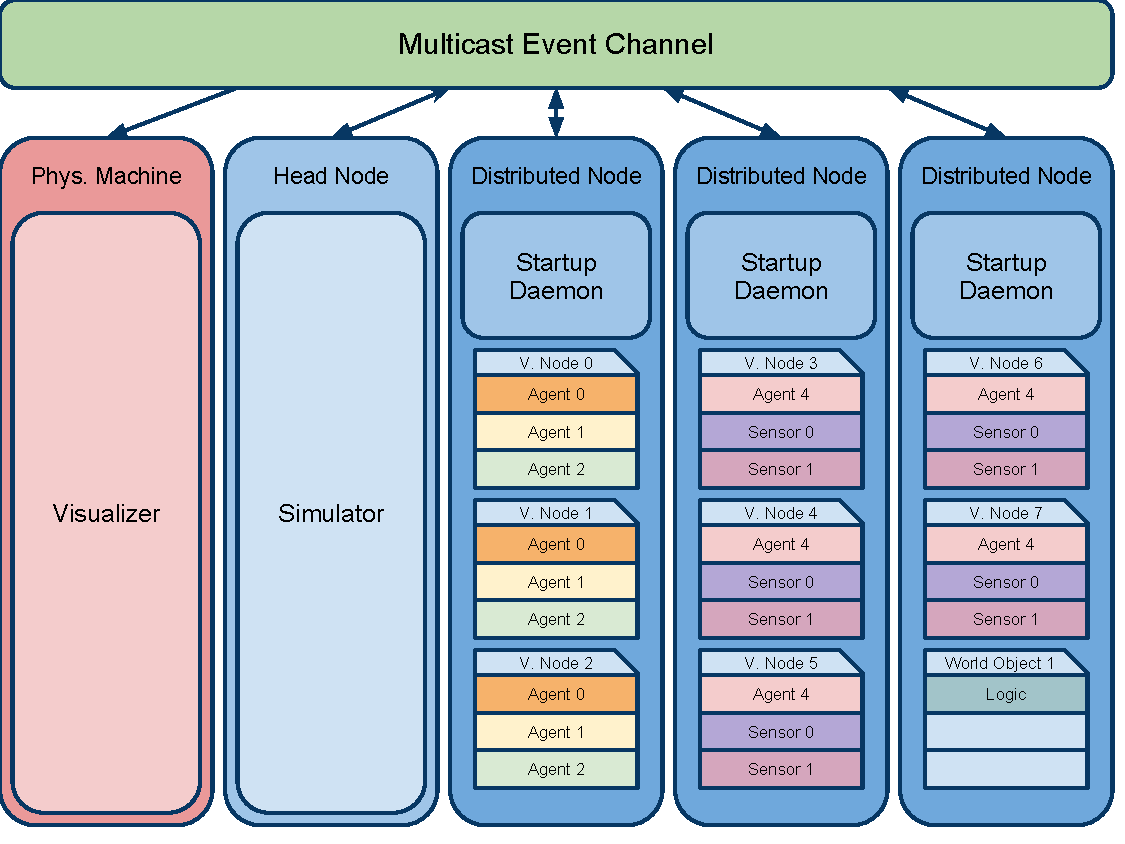
\includegraphics[scale=.6]{../initial-pres/arch.pdf}
    \caption{Distribution Diagram}
    \label{fig-distribution}
\end{figure}

\subsection{User Interface Overview}
AHOY is intentionally designed to provide no specific user interface in the traditional sense. Instead, it provides an extensive and comprehensive API, for creating a simulation, interacting with an experiment as it is running, monitoring events from a global viewpoint, and recording the results of an experiment for analysis. This ultimately offers flexibility for the end user, as separate, pre-existing interfaces can be modified to support AHOY's software API, or simply created from scratch to explicitly satisfy the user's needs. 

\subsection{Technologies Used}
The AHOY project is written entirely in Python, an interpreted, general-purpose high-level programming language. It does not depend on any external or libraries or packages, aside from those provided by the standard library. These include: the \texttt{sys} and \texttt{time} modules for standard system functions, the \texttt{math} library for advanced calculations, the \texttt{threading}, \texttt{signal} and \texttt{subprocess} for managing the distributed system, and the \texttt{pickle}, \texttt{socket} and \texttt{struct} modules for organizing the multicast event channel.

\section{Detailed System Design}

\subsection{Simulator Components}
\subsubsection{Simulation}
\begin{figure}
    \centering
    \begin{tikzpicture}
        \umlclass[xshift=-2cm]{simulation}{Simulation}{
            \umlattr{\#}{\_event\_api}{EventAPI}
            \umlattr{\#}{\_startup\_acks}{set(int)}
            \umlattr{\#}{\_comms\_engine}{CommsEngine}
            \umlattr{\#}{\_world}{World}
        }{
            \umlmethod{+}{\_\_init\_\_}{world\_inst : World, comms\_engine : CommsEngine}{void}
            \umlmethod{\#}{\_on\_ack\_startup}{event : Event}{void}
            \umlmethod{+}{get\_world}{}{World}
            \umlmethod{+}{start}{wait : int}{void}
            \umlmethod{+}{stop}{}{void}
        }
        \umlclass[below of=simulation, yshift=-2cm]{world}{World}{
            \umlattr{\#}{\_entities}{dict(String : Entity)}
            \umlattr{\#}{\_networks}{dict(String : Network)}
            \umlattr{\#}{\_event\_api}{EventAPI}
            \umlattr{\#}{\_agent\_mapping}{dict(int : int)}
        }{
            \umlmethod{+}{\_\_init\_\_}{}{void}
            \umlmethod{+}{\underline{from\_pickle}}{pickled : String}{World}
            \umlmethod{\#}{\_on\_entity\_move}{event : Event}{void}
            \umlmethod{+}{add\_entity}{entity : Entity}{void}
            \umlmethod{+}{get\_entity}{}{Entity}
            \umlmethod{+}{get\_entities}{}{list(Entity)}
            \umlmethod{+}{add\_network}{}{void}
            \umlmethod{+}{get\_network}{String}{Network}
            \umlmethod{+}{get\_networks}{}{list(Network)}
            \umlmethod{+}{get\_agent\_mapping}{}{dict(int : int)}
            \umlmethod{+}{initialize}{}{void}
            \umlmethod{+}{pickle}{}{String}
        }
        \path [draw, <-, >=open diamond] (simulation) -- (world)
            node [very near start, auto=right] {}
            node [very near end, auto=right] {};
    \end{tikzpicture}
    \caption{Class diagram for simulation}
    \label{fig-simulation}
\end{figure}
\subsubsection{World}
\subsubsection{EventAPI}

\subsubsection{StartupDaemon}
\begin{figure}
    \centering
    \begin{tikzpicture}
        \umlclass[xshift=-2cm]{startup}{StartupDaemon}{
            \umlattr{\#}{\_event\_api}{EventAPI}
            \umlattr{\#}{\_phys\_id}{int}
            \umlattr{\#}{\_running\_pids}{set(int)}
            \umlattr{\#}{\_running}{bool}
        }{
            \umlmethod{+}{\_\_init\_\_}{phys\_id : int}{void}
            \umlmethod{\#}{\_on\_startup}{event : Event}{void}
            \umlmethod{\#}{\_start\_entity\_process}{entity : Entity}{void}
            \umlmethod{\#}{\_on\_sim\_start}{event : Event}{void}
            \umlmethod{\#}{\_restart}{event : Event}{void}
            \umlmethod{+}{terminate\_all}{}{void}
            \umlmethod{+}{start}{}{void}
            \umlmethod{+}{stop}{}{void}
        }
    \end{tikzpicture}
    \caption{Class diagram for startup daemon}
    \label{fig-startupdaemon}
\end{figure}

\subsubsection{Entity}
\begin{figure}
    \centering
    \begin{tikzpicture}
        \umlclass[xshift=-2cm]{entity}{Entity \textit{$<<$Abstract$>>$}}{
            \umlattr{\#}{\_uid}{int}
            \umlattr{\#}{\_lat}{float}
            \umlattr{\#}{\_lon}{float}
            \umlattr{\#}{\_agl}{float}
            \umlattr{\#}{\_rcs}{float}
            \umlattr{\#}{\_event\_api}{EventAPI}
            \umlattr{\#}{\_world}{World}
            \umlattr{\#}{\_velocity}{(float, float, float)}
            \umlattr{\#}{\_sensors}{dict(String : Sensor)}
        }{
            \umlmethod{+}{\_\_init\_\_}{phys\_id : int}{void}
            \umlmethod{+}{\underline{from\_pickle}}{String}{Entity}
            \umlmethod{\#}{\_iterate\_move}{pos : (float, float, float), vel : float}{void}
            \umlmethod{+}{add\_sensor}{name : String, sensor : Sensor}{void}
            \umlmethod{+}{get\_sensor}{name : String}{Sensor}
            \umlmethod{+}{get\_rcs}{}{float}
            \umlmethod{+}{set\_rcs}{float}{void}
            \umlmethod{+}{get\_velocity}{}{(float, float, float)}
            \umlmethod{+}{set\_velocity}{vel : (float, float, float)}{void}
            \umlmethod{+}{get\_world}{}{World}
            \umlmethod{+}{set\_world}{world : World}{}
            \umlmethod{+}{get\_position}{}{(float, float, float)}
            \umlmethod{+}{set\_position}{pos : (float, float, float)}{}
            \umlmethod{+}{move}{pos : (float, float, float)}{}
            \umlmethod{+}{pickle}{}{String}
            \umlmethod{+}{get\_event\_api}{}{EventAPI}
            \umlmethod{+}{get\_uid}{}{int}
            \umlmethod{+}{initialize}{}{void}
            \umlmethod{+}{\textit{run}}{}{void}
        }

        \umlclass[minimum width=5cm, text width=8cm, yshift=-7cm, below left of=entity]{node}{Node}{
            \umlattr{\#}{\_interfaces}{list(Interface)}
            \umlattr{\#}{\_agents}{list(Agent)}
        }{
            \umlmethod{+}{\_\_init\_\_}{uid : int}{void}
            \umlmethod{\#}{\_on\_message}{event : Event, **kwds : dict}{void}
            \umlmethod{+}{get\_agent\_uids}{}{list(int)}
            \umlmethod{+}{add\_interface}{interface : Interface}{void}
            \umlmethod{+}{remove\_interface}{name : String}{void}
            \umlmethod{+}{get\_interface}{name : String}{Interface}
            \umlmethod{+}{get\_interfaces}{}{list(Interface)}
            \umlmethod{+}{add\_agent}{agent : Agent}{void}
            \umlmethod{+}{get\_interface\_on\_net}{network\_name : String}{Interface}
            \umlmethod{+}{send}{message : Message, src\_agent : Agent}{void}
            \umlmethod{+}{run}{}{void}
        }
        \umlclass[minimum width=5cm, text width=5cm, yshift=-6cm, below right of=entity]{scripted}{ScriptedEntity}{
            \umlattr{\#}{\_waypoints}{list((float, float, float))}
            \umlattr{\#}{\_vel}{float}
        }{
            \umlmethod{+}{\_\_init\_\_}{uid : int, waypoints : list((float, float, float)), vel : float}{void}
            \umlmethod{+}{run}{}{void}
        }
        \path [draw, <-, >=open triangle 45] (entity) -- (node)
            node [very near start, auto=right] {}
            node [very near end, auto=right] {};
        \path [draw, <-, >=open triangle 45] (entity) -- (scripted)
            node [very near start, auto=right] {}
            node [very near end, auto=right] {};
    \end{tikzpicture}
    \caption{Class diagram for entities}
    \label{fig-entities}
\end{figure}
\subsubsection{Built-in Entities}
\paragraph{Node}
\paragraph{ScriptedEntity}
\subsubsection{Startup Sequence}
\begin{figure}
  \centering

  \begin{sequencediagram}
    \newthread{sim}{Simulation}{Simulation}
    \newthread{mc}{Event Channel}{EventChannel}
    \newthread{startup1}{StartupDaemon 1}{StartupDaemon}
    \newthread{startupn}{StartupDaemon $n$}{StartupDaemon}

    \mess{sim}{StartupEvent}{mc}
    \begin{callself}{sim}{time.sleep()}{}
        \mess{mc}{StartupEvent}{startup1}
        \mess{mc}{\hspace*{3cm}StartupEvent}{startupn}
        \mess{startup1}{AckStartupEvent}{mc}
        \mess{mc}{AckStartupEvent}{sim}
        \mess{startupn}{\hspace*{3cm}AckStartupEvent}{mc}
        \mess{mc}{AckStartupEvent}{sim}
    \end{callself}
    \begin{callself}{sim}{allocate\_entities()}{}
    \end{callself}
    \mess{sim}{StartSimulationEvent}{mc}
    \mess{mc}{StartSimulationEvent}{startup1}
    \begin{callself}{startup1}{start\_entities()}{}
    \end{callself}
    \mess{mc}{\hspace*{3.7cm}StartSimulationEvent}{startupn}
    \begin{callself}{startupn}{start\_entities()}{}
    \end{callself}
  \end{sequencediagram}

  \caption{Startup sequence}
  \label{fig-startupseq}
\end{figure}
\subsection{Networking Components}
\subsubsection{Interface}
\begin{figure}
    \centering
    \begin{tikzpicture}
        \umlclass[]{interface}{Interface}{
            \umlattr{\#}{\_name}{String}
            \umlattr{\#}{\_owner\_node}{Node}
            \umlattr{\#}{\_recv\_callback}{function}
            \umlattr{\#}{\_network\_name}{String}
            \umlattr{\#}{\_power}{float}
        }{
            \umlmethod{+}{\_\_init\_\_}{name : String, owner\_node : Node, network : Network, power : float}{void}
            \umlmethod{\#}{\_on\_communication}{event : Event}{void}
            \umlmethod{+}{connect}{}{void}
            \umlmethod{+}{send}{message\_inst : Message, src\_agent : int}{void}
            \umlmethod{+}{set\_recv\_callback}{cb : function}{void}
            \umlmethod{+}{get\_owner}{}{Node}
            \umlmethod{+}{get\_network\_name}{}{String}
            \umlmethod{+}{get\_name}{}{String}
            \umlmethod{+}{get\_power}{}{float}
        }
    \end{tikzpicture}
    \caption{Class diagram for interfaces}
    \label{fig-interface}
\end{figure}
\subsubsection{CommsEngine}
\begin{figure}
    \centering
    \begin{tikzpicture}
        \umlclass[]{comms}{CommsEngine \textit{$<<$Abstract$>>$}}{
            \umlattr{\#}{\_event\_api}{EventAPI}
            \umlattr{\#}{\_simulation}{Simulation}
        }{
            \umlmethod{+}{\_\_init\_\_}{}{void}
            \umlmethod{\#}{\textit{\_on\_send}}{event : Event}{void}
            \umlmethod{+}{get\_node\_from\_agent}{agent\_uid : int}{int}
            \umlmethod{+}{set\_simulation}{simulation : Simulation}{void}
            \umlmethod{+}{get\_event\_api}{}{EventAPI}
            \umlmethod{+}{get\_simulation}{}{Simulation}
        }
        \eumlclass[minimum width=5cm, text width=6cm, below left of=comms, yshift=-2cm]{logloss}{LogLossCommsEngine}
        {
            \umlmethod{+}{\_\_init\_\_}{}{void}
            \umlmethod{\#}{\_on\_send}{event : Event}{void}
            \umlmethod{\#}{\_on\_movement}{event : Event}{void}
            \umlmethod{\#}{\_get\_rx\_power}{src\_uid : int, dest\_uid : int, src\_power : float}{float}
            \umlmethod{\#}{\_should\_deliver}{src\_uid : int, dest\_uid : int, src\_power : float, dest\_sensitivity : float}{bool}
        }
        \eumlclass[minimum width=5cm, text width=6cm, below right of=comms, yshift=-2cm]{ethernet}{EthernetCommsEngine}
        {
            \umlmethod{+}{\_\_init\_\_}{}{void}
            \umlmethod{\#}{\_on\_send}{event : Event}{void}
            \umlmethod{\#}{\_on\_movement}{event : Event}{void}
        }
        \path [draw, <-, >=open triangle 45] (comms) -- (logloss)
            node [very near start, auto=right] {}
            node [very near end, auto=right] {};
        \path [draw, <-, >=open triangle 45] (comms) -- (ethernet)
            node [very near start, auto=right] {}
            node [very near end, auto=right] {};
    \end{tikzpicture}
    \caption{Class diagram for communication engines}
    \label{fig-interface}
\end{figure}
\subsubsection{Built-in CommsEngines}
\paragraph{LogLossCommsEngine}
\paragraph{EthernetCommsEngine}

\subsection{Event Components}
\subsubsection{Event}
\begin{figure}
    \centering
    \scalebox{0.7}{
    \begin{tikzpicture}
        \eumlclass[]{event}{Event \textit{$<<$Abstract$>>$}}
        {
            \umlmethod{+}{\_\_init\_\_}{}{void}
            \umlmethod{+}{\underline{from\_pickle}}{pickled : String}{Event}
            \umlmethod{+}{pickle}{}{String}
        }
        \umlclass[minimum width=5cm, text width=5cm, xshift=-6cm, below of=event]{send}{CommunicationSendEvent}{
            \umlattr{\#}{\_src\_agent\_uid}{int}
            \umlattr{\#}{\_src\_iface\_name}{String}
            \umlattr{\#}{\_message}{Message}
            \umlattr{\#}{\_network}{String}
        }
        {
            \umlmethod{+}{\_\_init\_\_}{src\_agent\_uid : int, src\_iface\_name : String, message\_inst : Message, network : String}{void}
            \umlmethod{+}{get\_src\_agent\_uid}{}{int}
            \umlmethod{+}{get\_src\_iface\_name}{}{String}
            \umlmethod{+}{get\_message}{}{Message}
            \umlmethod{+}{get\_network}{}{String}
        }
        \umlclass[minimum width=5cm, text width=5cm, below of=event]{recv}{CommunicationRecvEvent}{
            \umlattr{\#}{\_src\_agent\_uid}{int}
            \umlattr{\#}{\_src\_iface\_name}{String}
            \umlattr{\#}{\_message}{Message}
            \umlattr{\#}{\_network}{String}
        }
        {
            \umlmethod{+}{\_\_init\_\_}{src\_agent\_uid : int, src\_iface\_name : String, message\_inst : Message, network : String}{void}
            \umlmethod{+}{get\_src\_agent\_uid}{}{int}
            \umlmethod{+}{get\_src\_iface\_name}{}{String}
            \umlmethod{+}{get\_message}{}{Message}
            \umlmethod{+}{get\_network}{}{String}
        }
        \umlclass[minimum width=5cm, text width=5cm, xshift=6cm, below of=event]{link}{LinkEvent}{
            \umlattr{\#}{\_up}{bool}
            \umlattr{\#}{\_uid\_1}{int}
            \umlattr{\#}{\_uid\_2}{int}
            \umlattr{\#}{\_network\_name}{String}
            \umlattr{\#}{\_pathloss}{float}
        }
        {
            \umlmethod{+}{\_\_init\_\_}{up : bool, uid\_1 : int, uid\_2 : int, network\_name : String, pathloss : float}{void}
            \umlmethod{+}{get\_up}{}{bool}
            \umlmethod{+}{get\_uid\_1}{}{int}
            \umlmethod{+}{get\_uid\_2}{}{int}
            \umlmethod{+}{get\_network\_name}{}{String}
            \umlmethod{+}{get\_pathloss}{}{float}
        }
        \umlclass[minimum width=5cm, text width=5cm, xshift=-6cm, above of=event]{move}{MoveEvent}{
            \umlattr{\#}{\_entity\_uid}{int}
            \umlattr{\#}{\_lat}{float}
            \umlattr{\#}{\_lon}{float}
            \umlattr{\#}{\_agl}{float}
            \umlattr{\#}{\_velocity}{float}
        }
        {
            \umlmethod{+}{\_\_init\_\_}{entity : Entity, lat : float, lon : float, agl : float, vel : float}{void}
            \umlmethod{+}{get\_uid}{}{int}
            \umlmethod{+}{get\_lat}{}{float}
            \umlmethod{+}{get\_lon}{}{float}
            \umlmethod{+}{get\_agl}{}{float}
            \umlmethod{+}{get\_velocity}{}{float}
        }
        \umlclass[minimum width=5cm, text width=5cm, above of=event]{start}{StartupEvent}{
            \umlattr{\#}{\_world}{World}
        }
        {
            \umlmethod{+}{\_\_init\_\_}{world : World}{void}
            \umlmethod{+}{get\_world}{}{World}
        }
        \umlclass[minimum width=5cm, text width=5cm, xshift=6cm, above of=event]{ackstart}{AckStartupEvent}{
            \umlattr{\#}{\_daemon\_id}{int}
        }
        {
            \umlmethod{+}{\_\_init\_\_}{daemon\_id : int}{void}
            \umlmethod{+}{get\_daemon\_id}{}{int}
        }
        \umlclass[minimum width=5cm, text width=5cm, xshift=-4cm, left of=event]{startsim}{StartSimulationEvent}{
            \umlattr{\#}{\_entity\_mapping}{dict(int : int)}
        }
        {
            \umlmethod{+}{\_\_init\_\_}{daemon\_id : int}{void}
            \umlmethod{+}{get\_mapping}{}{dict(int : int)}
        }
        \eumlclass[minimum width=5cm, text width=5cm, xshift=4cm, right of=event]{stop}{StopSimulationEvent}
        {
            \umlmethod{+}{\_\_init\_\_}{}{void}
        }

        \path [draw, <-, >=open triangle 45] (event) -| (send);
        \path [draw, <-, >=open triangle 45] (event) -- (recv);
        \path [draw, <-, >=open triangle 45] (event) -| (link);
        \path [draw, <-, >=open triangle 45] (event) -| (move);
        \path [draw, <-, >=open triangle 45] (event) -- (start);
        \path [draw, <-, >=open triangle 45] (event) -| (ackstart);
        \path [draw, <-, >=open triangle 45] (event) -- (startsim);
        \path [draw, <-, >=open triangle 45] (event) -- (stop);
    \end{tikzpicture}}
    \caption{Class diagram for events}
    \label{fig-events}
\end{figure}

\subsubsection{Built-in Events}
Built-in events are specific Event classes provided by default to any emulation. These embody the basic events for a network simulation, but users are encouraged to develop and add their own as well.
\paragraph{LinkEvent}{Published when a network link between two entities changes within the simulation.}

\attributes{
    \attribute{\_up}{bool}{Whether the link is currently up (connected)}
    \attribute{\_uid\_1}{int}{UID of the first node which makes up the link}
    \attribute{\_uid\_2}{int}{UID of the second node which makes up the link}
    \attribute{\_network\_name}{string}{The network that the link exists on}
    \attribute{\_pathloss}{float}{Pathloss value for wireless links}
}

\operations{
    \operation{\_\_init\_\_(up, uid\_1, uid\_2, network\_name, pathloss)}
    {
        \begin{itemize*}
            \item \texttt{up}: Whether the link is up
            \item \texttt{uid\_1}: The UID of the first node
            \item \texttt{uid\_2}: The UID of the second node
            \item \texttt{network\_name}: The name of the network
            \item \texttt{pathloss}: The pathloss value, if relevant
        \end{itemize*}
    }{None}{Instantiates a new link action}
    \operation{get\_up()}{None}{Link State}{Gets whether or not the link is connected}
    \operation{get\_uid1()}{None}{First Agent UID}{Gets the UID of the first node in the link}
    \operation{get\_uid2()}{None}{Second Agent UID}{Gets the UID of the second node in the link}
    \operation{get\_network\_name()}{Network Name}{None}{Gets the name of the network}
    \operation{get\_pathloss()}{None}{Pathloss Value}{Gets the pathloss value for wireless links}
}

\paragraph{CommunicationSendEvent}{Published when an entity sends a message within the simulation.}

\attributes{
    \attribute{\_src\_agent\_uid}{int}{UID of the entity that is the source of the message}
    \attribute{\_src\_iface\_name}{string}{Interface name that the message is sent on}
    \attribute{\_message}{Message}{An instance of the message that is sent}
    \attribute{\_network}{string}{The network that the interface is a part of}
}

\operations{
    \operation{\_\_init\_\_(src\_agent\_uid, src\_iface\_name, message\_inst, network)}
    {
        \begin{itemize*}
            \item \texttt{src\_agent\_uid}: UID of the sending agent
            \item \texttt{src\_iface\_name}: Name of the interface
            \item \texttt{message\_inst}: Instance of the message being sent
            \item \texttt{network}: Name of the network
        \end{itemize*}
    }{None}{Instantiates a new communication send action}
    \operation{get\_src\_agent\_uid()}{None}{Source Agent UID}{Gets the UID of the source entity that sent the message}
    \operation{get\_src\_iface\_name()}{None}{Source Interface Name}{Gets the name of the interface the message was sent on}
    \operation{get\_message()}{None}{Message}{Gets the entirety of the message}
    \operation{get\_network()}{None}{Network Name}{Gets the network the message was sent on}
}

\paragraph{CommunicationRecvEvent}{Published when an entity receives a message within the simulation.}

\attributes{
    \attribute{\_src\_agent\_uid}{int}{UID of the entity that is the source of the message}
    \attribute{\_src\_iface\_name}{string}{Interface name that the message is sent on}
    \attribute{\_message}{Message}{An instance of the message that is sent}
    \attribute{\_network}{string}{The network that the interface is a part of}
}

\operations{
    \operation{\_\_init\_\_(src\_agent\_uid, src\_iface\_name, message\_inst, network)}
    {
        \begin{itemize*}
            \item \texttt{src\_agent\_uid}: UID of the sending agent
            \item \texttt{src\_iface\_name}: Name of the interface
            \item \texttt{message\_inst}: Instance of the message being sent
            \item \texttt{network}: Name of the network
        \end{itemize*}
    }{None}{Instantiates a new communication receive action}
    \operation{get\_src\_agent\_uid()}{None}{Source Agent UID}{Gets the UID of the source entity that sent the message}
    \operation{get\_src\_iface\_name()}{None}{Source Interface Name}{Gets the name of the interface the message was sent on}
    \operation{get\_message()}{None}{Message}{Gets the entirety of the message}
    \operation{get\_network()}{None}{Network Name}{Gets the network the message was sent on}
}

\paragraph{EntityMoveEvent}{Published when an entity moves within the simulation.}

\attributes{
    \attribute{\_entity\_uid}{int}{UID of the entity that moved}
    \attribute{\_lat}{float}{Latitude of new location}
    \attribute{\_lon}{float}{Longitude of new location}
    \attribute{\_agl}{float}{AGL of new location}
    \attribute{\_velocity}{float}{Velocity of movement}
}

\operations
{
    \operation{\_\_init\_\_(entity, lat, lon, agl, velocity)}
    {
        \begin{itemize*}
            \item \texttt{entity}: Instance of entity that moved
            \item \texttt{lat}: Latitude of new location
            \item \texttt{lon}: Longitude new location
            \item \texttt{agl}: AGL of new location
            \item \texttt{velocity}: Velocity of movement
        \end{itemize*}
    }{None}{Instantiates a new movement action}
    \operation{get\_uid()}{None}{UID}{Gets the UID of the entity that moved}
    \operation{get\_lat()}{None}{Latitude}{Gets the new latitude of the entity that moved}
    \operation{get\_lon()}{None}{Longitude}{Gets the new longitude of the entity that moved}
    \operation{get\_agl()}{None}{AGL}{Gets the new AGL of the entity that moved}
    \operation{get\_velocity()}{None}{Velocity}{Gets the velocity of the entity that moved}
}

\paragraph{StartupEvent}
\paragraph{AckStartupEvent}
\paragraph{StartSimulationEvent}
\paragraph{StopSimulationEvent}

\subsection{Agent Components}
\subsubsection{Agent}
\begin{figure}
    \centering
    \begin{tikzpicture}
        \umlclass[xshift=-2cm]{action}{Agent \textit{$<<$Abstract$>>$}}{
            \umlattr{\#}{\_owner\_node}{Node}
            \umlattr{\#}{\_uid}{int}
            \umlattr{\#}{\_behaviors}{dict(Event : list([precondition, action]))}
        }{
            \umlmethod{+}{\_\_init\_\_}{owner\_uid, uid}{void}
            \umlmethod{\#}{\_on\_event}{event : Event}{void}
            \umlmethod{\#}{\_init\_behavior}{void}{void}
            \umlmethod{+}{get\_uid}{}{int}
            \umlmethod{+}{get\_owner\_node}{}{Node}
            \umlmethod{+}{on\_message}{event : Event}{void}
            \umlmethod{+}{start}{}{void}
            \umlmethod{+}{add\_behavior}{behavior : (precond, event, action)}{void}
            \umlmethod{+}{remove\_behavior}{behavior : (precond, event, action)}{void}
            \umlmethod{+}{\textit{run}}{}{void}
        }
    \end{tikzpicture}
    \caption{Class diagram for agents}
    \label{fig-agents}
\end{figure}
\subsubsection{Condition}
\begin{figure}
    \centering
    \begin{tikzpicture}
        \eumlclass[xshift=-2cm]{condition}{Condition \textit{$<<$Abstract$>>$}}
        {
            \umlmethod{+}{\_\_init\_\_}{}{void}
            \umlmethod{+}{\textit{is\_met}}{event : Event}{bool}
        }
    \end{tikzpicture}
    \caption{Class diagram for conditions}
    \label{fig-condition}
\end{figure}

\subsubsection{Action}
\begin{figure}
    \centering
    \begin{tikzpicture}
        \eumlclass[]{action}{Action \textit{$<<$Abstract$>>$}}
        {
            \umlmethod{+}{\_\_init\_\_}{}{void}
            \umlmethod{+}{\textit{perform}}{}{void}
        }
        \umlclass[below of=action]{move}{Move}{
            \umlattr{\#}{\_entity}{int}
            \umlattr{\#}{\_lat}{float}
            \umlattr{\#}{\_lon}{float}
            \umlattr{\#}{\_agl}{float}
        }
        {
            \umlmethod{+}{\_\_init\_\_}{entity : int, lat : float, lon : float, agl : float}{void}
            \umlmethod{+}{perform}{}{void}
        }
        \path [draw, <-, >=open triangle 45] (action) -- (move)
            node [very near start, auto=right] {}
            node [very near end, auto=right] {};
    \end{tikzpicture}
    \caption{Class diagram for actions}
    \label{fig-actions}
\end{figure}
\subsubsection{Built-in Actions}
\paragraph{Move}

\subsection{Sensor Components}
\subsubsection{Sensor}
\begin{figure}
    \centering
    \begin{tikzpicture}
        \umlclass[]{sensor}{Sensor \textit{$<<$Abstract$>>$}}{
            \umlattr{\#}{\_subscribers}{list(Entity)}
        }
        {
            \umlmethod{+}{\_\_init\_\_}{}{void}
            \umlmethod{\#}{\_publish\_data}{event : Event}{void}
            \umlmethod{+}{subscribe}{callback : function}{void}
            \umlmethod{+}{\textit{run}}{}{void}
        }
        \umlclass[below of=sensor]{radar}{RadarSensor}{
            \umlattr{\#}{\_trans\_power}{float}
            \umlattr{\#}{\_trans\_freq}{float}
            \umlattr{\#}{\_gain}{float}
            \umlattr{\#}{\_aperture}{float}
            \umlattr{\#}{\_prop\_fac}{float}
            \umlattr{\#}{\_dwell\_time}{float}
            \umlattr{\#}{\_angle}{float}
        }
        {
            \umlmethod{+}{\_\_init\_\_}{}{void}
            \umlmethod{\#}{\_publish\_data}{event : Event}{void}
            \umlmethod{+}{subscribe}{callback : function}{void}
            \umlmethod{+}{run}{}{void}
        }

        \path [draw, <-, >=open triangle 45] (sensor) -- (radar)
            node [very near start, auto=right] {}
            node [very near end, auto=right] {};
    \end{tikzpicture}
    \caption{Class diagram for sensors}
    \label{fig-sensors}
\end{figure}
\subsubsection{Built-in Sensors}
\paragraph{RadarSensor}

\subsection{Utility Components}
\subsubsection{Geo}
\begin{figure}
    \centering
    \begin{tikzpicture}
        \eumlclass[xshift=-2cm]{geo}{Geo}
        {
            \umlmethod{+}{\underline{haver\_distance}}{lat1 : float, lon1 : float, lat2 : float, lon2 : float}{float}
            \umlmethod{+}{\underline{linear\_distance}}{lat1 : float, lon1 : float, lat2 : float, lon2 : float}{float}
            \umlmethod{+}{\underline{sph\_to\_lin}}{lat : float, lon : float, agl : float}{(float, float, float)}
            \umlmethod{+}{\underline{lin\_to\_sph}}{x : float, y : float, z : float}{(float, float, float)}
            \umlmethod{+}{\underline{linear\_to\_degree}}{lat : float, lon : float, lat\_km : float, lon\_km : float}{float}
            \umlmethod{+}{\underline{loc\_from\_bearing\_dist}}{lat : float, lon : float, bearing : float, dist : float}{float}
        }
    \end{tikzpicture}
    \caption{Class diagram for geographic utilities}
    \label{fig-condition}
\end{figure}
\end{document}
